\chapter{Evaluation}\label{chapter:evaluation}

In this section we provide an extensive experimental evaluation of the HyPer k-Means operator. We compare the different  HyPer implementations to each other as well as to state-of-the-art technologies of clustering data. 
All experiments have been performed on a workstation equipped with sixteen 2.93 GHz CPUs and 64 MB of main memory.


\section{Data Sets}
To provide an objective comparison the execution time per iteration is measured. Therefore the different technologies can be compared fairly and random initialization and internal improvments for faster convergence do not affect the outcome. For the experiments a real world data set is used and four synthetic data sets have been generated. The synthetic data sets represent a high dimensional, a medium size, a medium sized high dimensional and a large size data set as shown in~\autoref{tab:dataset}. All are generated on a uniform random distribution. The data sets are selected in a way that most real world use cases are covered.

\begin{table}[htsb]
  \caption[Data Sets]{Data Sets.}\label{tab:dataset}
  \centering
  \begin{tabular}{l l l l l}
    \toprule
      & Instances & Dimensions & Size (byte) & Size (Gigabyte) \\
    \midrule
      3D Network        & 434874    & 4     & 20673913 & 0.019 \\
      High Dimensional  & 50000     & 50    & 10000000 & 0.009 \\
      Medium Size       & 15M       & 4     & 240000000 & 0.22 \\
      Medium Size HD    & 15M       & 50    & 3000000000 & 2.79 \\
      Large Size        & 150M      & 10    & 6000000000 & 5.59 \\
    \bottomrule
  \end{tabular}
\end{table}



\begin{itemize} 
\item 3D Network: The first data set contains the 3D spatial road network data of a road network in North Jutland, Denmark~\parencite{3dnet}. It is a real world data set available at the UCI Machine Learning Repository~\parencite{uci} and consists of 434874 data points in four dimensions: An id for the road segment, the latitude, the longitude and the altitude of the segment. The id is a large integer, the other dimensions are floating point numbers. The size of the data set is 20,673,913 bytes, therefore it is a rather small data set.

\item High Dimensional: The second dataset is a synthetic data set. It consists of 50000 data points in 50 dimensions. All dimensions are floating point numbers. The size of the data set is 10000000 bytes, hence also a rather small data set, but this time high dimensional.

\item Medium Size: The data set consists of 15 million data points in four dimensions. It is also a synthetic data set generated, all four dimensions containing floating point numbers. The size of the data set is 240000000 bytes and presents the medium size data set in this experiment section.

\item Medium Size HD: The Medium Size HD data set is generated the same way as the Medium Size data set. Instead of four dimensions, this time 50 dimension have been generated. This leads to a growth from 0.22 GB to 2.79 GB.  

\item Large Size: Finally, the large data set consists of 150 million data points in ten dimension. It is also synthetically generated by a random uniform distribution of floating point numbers. The size of the data set is 5.59 GB.
\end{itemize} 



\section{Used Tools}

As already described in chapter \ref{chapter:related}, there exist many tools for data mining. In this section we look at a selection of tools implementing the k-Means clustering algorithm we are using to compare with our k-Means HyPer operator. To make the results comparable in a fair manner, we use only tools that give enough information about the clustering process, e.g. number of iterations, total cost and most important, the applied algorithm. Not all tools are implementing the Lloyd algorithm, e.g. the default version of R is the Hartigan-Wong algorithm, an improvement over the standard Lloyd algorithm.
\\
Since k-Means is a non-deterministic algorithm, the number of iterations is the most important criteria to make the results comparable. Running time of k-Means depends almost entirely on the number of iterations the algorithm has to make, which depends on the non-deterministic initialization. Therefore the running time should be relative to the number of iterations.
\\
Unfortunately, neither ELKI nor Scipy’s k-Means implementation provide the number of iterations as output. Therefore, a fair comparison is not possible. Fortunately, Weka, R and Julia provide good configuration possibilities as well as a result set that contains information about the number of iterations. Wile Weka is written in Java, R and Julia are both written in a high level language. Even though, critical code parts are implemented in C, C++ and Fortran for better performance results, without the overhead of an entire database system behind. Therefore it will be interesting to compare HyPer Weka, R and Julia.
\\
The usability and user experience among R and Julia is very similar: Both can be run as interactive program or as script using a functional language. Various plotting functionalities are provided. Both tools provide a CSV reader to import our data. HyPer can be run as interactive console program or as script, too, and provides efficient CSV loading~\cite{hypercsv}. Weka can be run from the command line, too, directly in Java programs or with its graphical user interface. However, internally Weka uses a custom arff format for its algorithms. When using the GUI converting the original data (in our case in CSV format) to the arff format happens in a preprocessing step and feels fairly natural. When using the command line or Java programs on a csv file, this file has to be preprocessed to the arff format, even though no further preprocessing is necessary. This takes time and is not as convenient as the other tools.
\\
Regarding the performance, Weka shows very disappointing results compared to Julia, R and HyPer, as depicted in~\autoref{tab:weka_final}. The table shows the median, the 90th and the 95th percentile running time per iteration for one iteration after 100 runs for $k = 3, 10$ and $20$. Comparing the results to the other tools Weka performs poorly. On the network data set, Weka is slower by a factor of 7 compared to the Julia implementation, which is the slowest on that data set. On the high dimensional data set, the HyPer C++ implementation shows the worst results, however, Weka is slower by a factor of around 6. As last test, the medium size data set was run against Weka, and it is slower by a factor of 10 for $k = 3$, 8 for $k = 10$ and 7 for $k = 20$ compared to Julia, the slowest one regarding this data set. Because of this tremendous differences in running time, we decided not to include Weka in the following performance section and only compare the performance to R and Julia.

\begin{table}[htsb]
  \caption[Weka Results - Time per Iteration]{Weka Results - Time per Iteration.}
  \label{tab:weka_final}
  \centering
  \begin{tabular}{l l l l l l l l l l }
    \toprule
      & \multicolumn{3}{c}{Network 3D} & \multicolumn{3}{c}{High Dimensional} & \multicolumn{3}{c}{Medium Size}  \\
      k & 3 & 10 & 20 & 3 & 10 & 20 & 3 & 10 & 20 \\
    \midrule
      50  & 1.39 & 1.54 & 1.93 & 1.08 & 1.39 & 1.90 & 54.01 & 58.25 & 71.11 \\
      90  & 1.48 & 1.60 & 2.02 & 1.16 & 1.44 & 1.98 &59.16 & 62.54 & 87.16 \\
      95  & 1.49 & 1.61 & 2.06 & 1.19 & 1.46 & 2.01 & 59.79 & 64.31 & 88.54 \\
    \bottomrule
  \end{tabular}
\end{table}



\section{Serial Implementation}\label{section:serial}

In this section we compare the two serial HyPer k-Means implementations: The C++ driven and the LLVM driven approach. For comparison we consider the compilation and the execution time. The compilation time is the time for generating LLVM code, while the execution time is the execution of the k-Means algorithm. Since the compilation time can be seen as a one-time setup time, we expect the execution time to be much larger. 
\\
For each data set, the two HyPer implementations are tested for 3,10 and 20 clusters. For each cluster number the algorithms was executed 100 times with a maximum number of iterations of 10. As result, the median time per iterations in seconds is stated. For better comparability the compilation time is also relative to the number of iterations, even though it does not change for a higher number of iterations.
\\
~\autoref{tab:network_serial} shows the result of the two serial implementations for the network data set. The compilation time is independent of the cluster number $k$ and does not differ among the C++ implementation and the LLVM version. In contrast the execution time increases as the cluster number $k$ increases. This is true for both implementations. For better visualization, ~\autoref{fig:hyper_network} depicts the same result as stacked bar charts.

\begin{table}[htsb]
  \caption[3D Network - Time per Iteration]{3D Network - Time per Iteration.}\label{tab:network_serial}
  \centering
  \begin{tabular}{l l l l l}
    \toprule
      & HyPer C++ & & HyPer LLVM & \\
      k & compilation[s] & execution[s] & compilation[s] & execution[s] \\
    \midrule
      3 & 0.0050 & 0.0680 & 0.0046 & 0.0171 \\
      10 & 0.0044 & 0.0947 & 0.0046 & 0.0502 \\
      20 & 0.0045 & 0.1391 & 0.0046 & 0.0901 \\
    \bottomrule
  \end{tabular}
\end{table}



 While the compilation time is low and constant, the execution time differs among implementation. In particular for $k = 3$, the execution time of the C++ version is almost four times the execution time of the LLVM version. For $k = 10$ it is two times the execution time and for $k = 20$ it is 1.5 times, respectively. On the other hand that means that for a larger cluster number $k$, the LLVM execution time grows  faster than the execution time of the C++ version. Actually, from $k = 3$ to $k = 10$, the LLVM version grows by a factor of 2.9, while the C++ grows by 1.4. From $k = 3$ to $k = 20$ the growth is even more significant, from factor 2 for the C++ version to 5.3 for the LLVM version.


\begin{figure}[htsb]
  \centering
  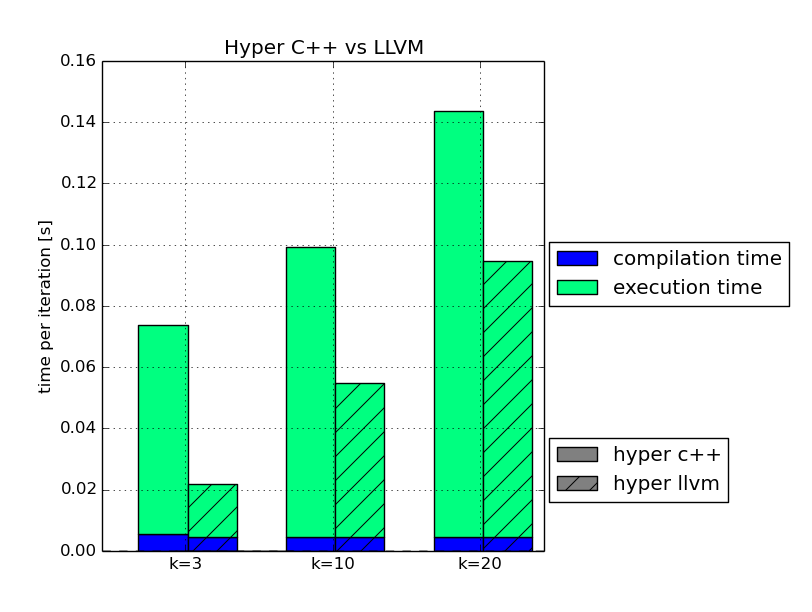
\includegraphics[scale=0.4, trim="0cm 1.5cm 0cm 0cm"]{figures/charts/hyper_network}
  \caption[3D Network - Time per Iteration]{3D Network - Time per Iteration.}
  \label{fig:hyper_network}
\end{figure}

This gives us the first interesting results. Although the C++ version is implementing k-Means using LLVM only for generated functions, the compilation time does not differ to the LLVM version, where not only the functions but also the entire algorithm is written in LLVM. Nevertheless, the functions for computing the distance and updating the centers are generated in LLVM for both implementations which is an explanation for the similar compilation times. In C++ these functions are generated as functions callable from C++, while in the LLVM version, the code is directly embedded into an LLVM program structure. The difference between the two seems to be insignificant.
\\
Regarding the execution time, the LLVM version is much faster than the C++ version. One reason is that the C++ implementation has many function calls between the \texttt{compile time} and the \texttt{runtime system}. For the LLVM system these calls are not necessary and the data remains in the CPU registers. The second advantage is that the entire algorithm is compiled in LLVM code resulting in a very efficient code, optimized on a lower level than even possible with C++ code.


\begin{table}[htsb]
  \caption[High Dimensional - Time per Iteration]{High Dimensional - Time per Iteration.}\label{tab:hd_serial}
  \centering
  \begin{tabular}{l l l l l}
    \toprule
      & HyPer C++ & & HyPer LLVM & \\
      k & compilation[s] & execution[s] & compilation[s] & execution[s] \\
    \midrule
      3  & 0.1278 & 0.0522 & 0.0933 & 0.0327 \\
      10 & 0.1287 & 0.1171 & 0.0933 & 0.0706 \\
      20 & 0.1299 & 0.2070 & 0.0933 & 0.1252 \\
    \bottomrule
  \end{tabular}
\end{table}

~\autoref{tab:hd_serial} shows the result of the same experiment with the high dimensional data set. In contrary to the network data set the compilation time is slightly different between the C++ and the LLVM implementation. Furthermore for both versions the compilation time is larger than the execution time for $k = 3$ and almost equal for $k = 10$. Only for $k = 20$ the execution time is larger than the compilation time, as depicted in~\autoref{fig:hyper_50000}.

\begin{figure}[htsb]
  \centering
  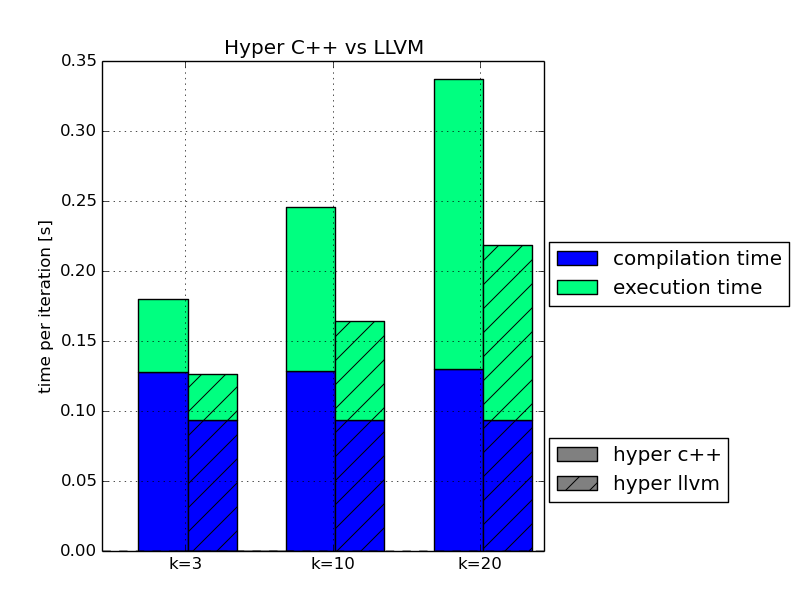
\includegraphics[scale=0.4, trim="0cm 1.5cm 0cm 0cm"]{figures/charts/hyper_50000}
  \caption[High Dimensional - Time per Iteration]{High Dimensional - Time per Iteration.}
  \label{fig:hyper_50000}
\end{figure}

Again, the compilation time stays constant for different values of $k$. The increase of compilation time is induced by the high dimensionality: For each dimension additional code has to be generated. Therefore a data set with four dimension is faster to compile than a data set with 50 dimensions. 
The difference in the running time is similar to the network data set even though the increase in performance is not as significant. For $k = 3$, LLVM is faster by a factor 1.6 and for $k = 10$ and $k = 20$ by facor 1.7. This time the increase in execution time is strongly correlated. From $k = 3$ to $k = 10$, the LLVM version and the C++ version grow by a factor of 2.2. From $k = 3$ to $k = 10$, the LLVM version grows by a factor of 4, while the C++ grows by 3.8.
\\
Interestingly, ten iterations terminate much quicker for the network data set than for the high dimensional data set, even though the network set is 2.1 times as large as the high dimensional data set. Even if we omit the compilation time which stays constant for a growing number of iterations, the execution time of the network data set is only for the C++ implemenation and $k = 3$ slower than the high dimensional data set. That shows us that our implementation performs much better for low dimensional data sets.
\\
\\
~\autoref{tab:med_serial} and ~\autoref{tab:med_hd_serial} show the same experiment for larger data sets. Both consist of 15 million instances, the first of four dimensions and the second of 50 dimensions. The compilation time of the medium size data set is similar to the network data set since both consist of four dimensions. The same is true for the medium size high dimensional data set and the smaller high dimensional data set. This proves that the compilation time is independent on the data size and only affect by the number of dimensions. However, as the number of instances is growing, the compilation time is not a significant factor for the overall execution time, as~\autoref{fig:hyper_15Mxhd} shows: The compilation time is not even visible plotting the data as barcharts as before.

\begin{table}[htsb]
  \caption[Medium Size - Time per Iteration]{Medium Size - Time per Iteration.}
  \label{tab:med_serial}
  \centering
  \begin{tabular}{l l l l l}
    \toprule
      & HyPer C++ & & HyPer LLVM & \\
      k & compilation[s] & execution[s] & compilation[s] & execution[s] \\
    \midrule
      3  & 0.0041 & 2.3779 & 0.0047 & 0.9191 \\
      10 & 0.0041 & 3.2856 & 0.0047 & 2.1001 \\
      20 & 0.0041 & 4.6765 & 0.0047 & 3.4518 \\
    \bottomrule
  \end{tabular}
\end{table}


\begin{table}[htsb]
  \caption[Medium Size High Dimensional - Time per Iteration]{Medium Size High Dimensional - Time per Iteration.}
  \label{tab:med_hd_serial}
  \centering
  \begin{tabular}{l l l l l}
    \toprule
      & HyPer C++ & & HyPer LLVM & \\
      k & compilation[s] & execution[s] & compilation[s] & execution[s] \\
    \midrule
      3  & 0.1127 & 16.2787 & 0.0935 & 10.3302 \\
      10 & 0.1127 & 34.0051 & 0.0935 & 22.0209 \\
      20 & 0.1126 & 59.2904 & 0.0935 & 38.7046 \\
    \bottomrule
  \end{tabular}
\end{table}

Obviously the execution time for the high dimensional data set is much larger again. For the C++ implementation the execution time is increased by a factor of 6.8 for $k = 3$, 10.3 for $k = 10$ and 12.6 for $k = 20$. For the LLVM implementation it is 11.2, 10.5, 11.2, respectively. Since the high dimensional data set is actually larger by a factor of 12.7, the values are strongly correlated to the growth of the data set.

\begin{figure}[htsb]
  \centering
  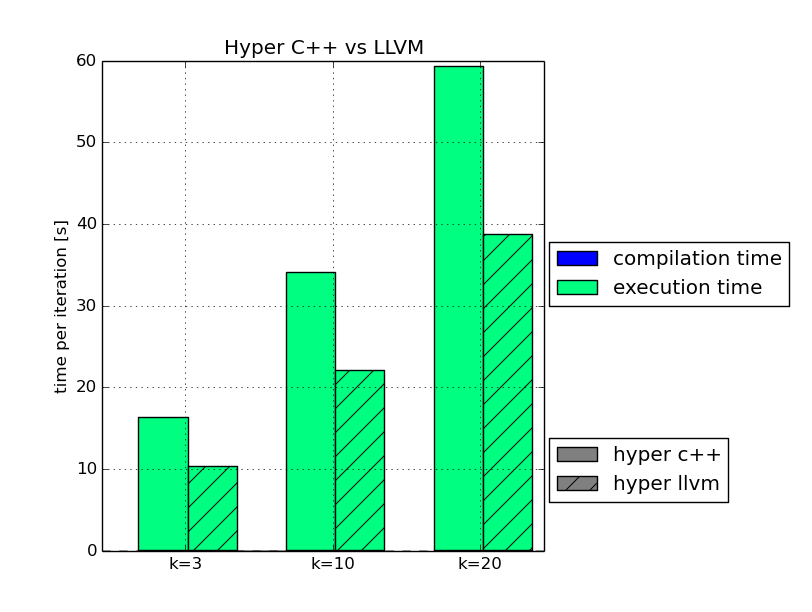
\includegraphics[scale=0.4, trim="0cm 1.5cm 0cm 0cm"]{figures/charts/hyper_15Mxhd}
  \caption[Medium Size High Dimensional - Time per Iteration]{Medium Size High Dimensional - Time per Iteration.}
  \label{fig:hyper_15Mxhd}
\end{figure}


~\autoref{tab:large_serial} shows the same experiment for the large data set. The data set consists of ten dimensions and therefore the compilation time increases compared to the data sets with four dimensions by a factor of around 2. Since the data set has a size of 5.59 GB the difference in the execution time is very significant. Again, the LLVM implementation is faster by around 20 seconds independent of the cluster number $k$.



\begin{table}[htsb]
  \caption[Large Size - Time per Iteration]{Large Size - Time per Iteration.}
  \label{tab:large_serial}
  \centering
  \begin{tabular}{l l l l l}
    \toprule
      & HyPer C++ & & HyPer LLVM & \\
      k & compilation[s] & execution[s] & compilation[s] & execution[s] \\
    \midrule
      3  & 0.0088 & 37.2804 & 0.0097 & 18.3734 \\
      10 & 0.0088 & 62.0034 & 0.0097 & 40.4783 \\
      20 & 0.0191 & 92.5868 & 0.0097 & 67.2364 \\
    \bottomrule
  \end{tabular}
\end{table}


In conclusion the compilation time is not affected if the number of instances gets large but only if the number of dimensions grows. The compilation time is similar between the LLVM version and the C++ version. Usually, the execution time outnumbers the compilation time by several factors. The only exception is the small, high dimensional data set as shown in the experiment. Here, the compilation time can be slower than the execution time.
\\
Furthermore the execution time grows by number of instances and is much faster for the LLVM implementation. With equality regarding the compilation and a performance decrease in execution time the LLVM version was for all experiments the best choice regarding the running time of the k-Means algorithm.


\section{Performance Test}\label{section:performance}

In this section we compare our serial HyPer implementations with Weka, R and Julia’s implementation of the k-Means algorithm. As algorithm, the Lloyd algorithm with a maximum iteration number of ten is chosen. Apart from the large data set, the algorithm is executed 100 times for $k = 3, 10$ and $20$, respectively. For the large data set, the algorithm is executed ten times. The result is then presented as the execution time per iteration. For each algorithm the median, the 90th percentile and the 95th percentile are given for every $k$. 
\\
\begin{table}[htsb]
  \caption[3D Network - Time per Iteration]{3D Network - Time per Iteration.}
  \label{tab:network_all1}
  \centering
  \begin{tabular}{l l l l l l l l l l l l l}
    \toprule
      & \multicolumn{3}{c}{Julia} & \multicolumn{3}{c}{R} & \multicolumn{3}{c}{HyPer C++} & \multicolumn{3}{c}{HyPer LLVM}  \\
      k & 3 & 10 & 20 & 3 & 10 & 20 & 3 & 10 & 20 & 3 & 10 & 20 \\
    \midrule
      50  & 0.21 & 0.22 & 0.29 & 0.03 & 0.04 & 0.08 & 0.08 & 0.10 & 0.14 & 0.02 & 0.06 & 0.10 \\
      50  & 0.27 & 0.30 & 0.32 & 0.06 & 0.06 & 0.10 & 0.09 & 0.12 & 0.20 & 0.03 & 0.06 & 0.10 \\
      50  & 0.31 & 0.35 & 0.35 & 0.08 & 0.07 & 0.11 & 0.10 & 0.13 & 0.22 & 0.03 & 0.06 & 0.10 \\
    \bottomrule
  \end{tabular}
\end{table}

\begin{figure}[htsb]
  \raggedleft
  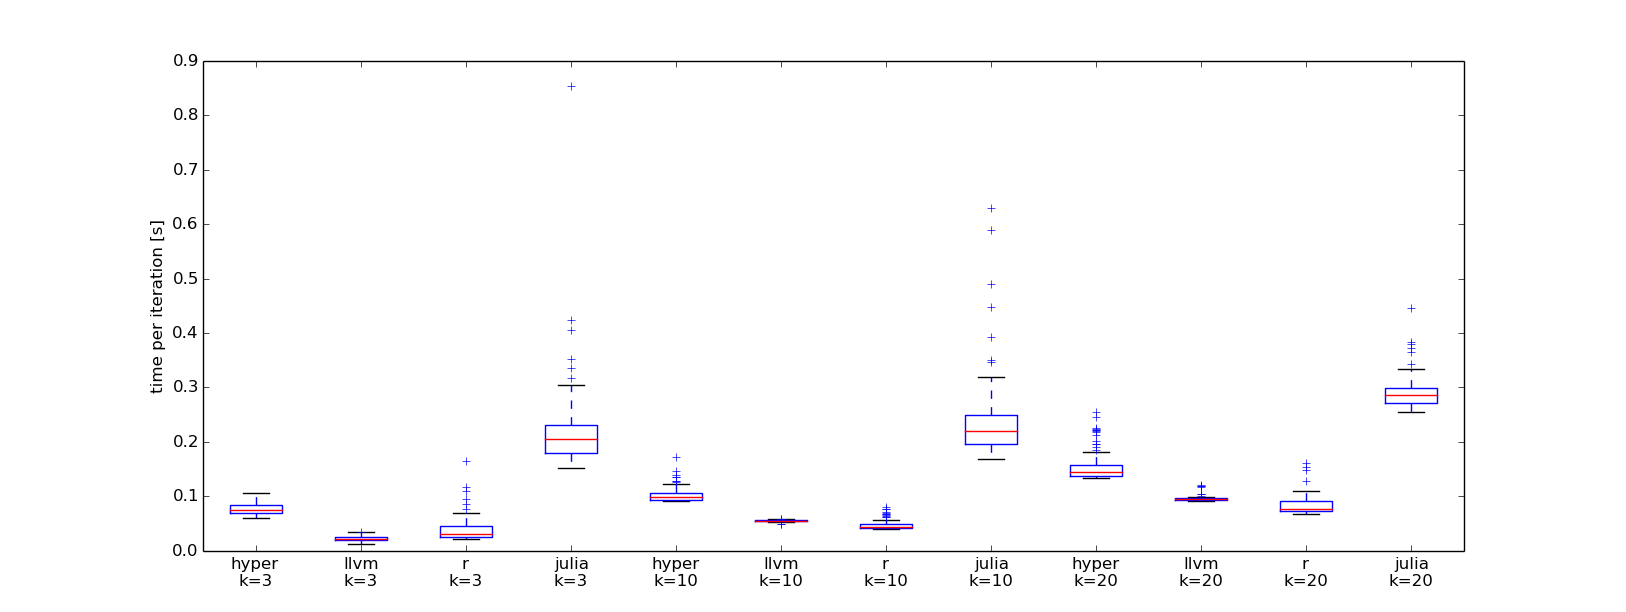
\includegraphics[scale=0.4, trim="0cm 1cm 0cm 0cm"]{figures/charts/network_all}
  \caption[3D Network - Time per Iteration]{3D Network - Time per Iteration.}
  \label{fig:network_all}
\end{figure}

The result is presented in~\autoref{tab:network_all1}. We already know that the HyPer LLVM implementation outnumbers the C++ version. For the median, the LLVM implementation is 3.4, 1.8 and 1.5 times faster for $k = 3, 10$ and $20$. Julia is the slowest, our LLVM implementation is 9.5, 4.0 and 3.1 for $k = 3, 10, 20$ times faster. Only the R implementation can compete with our HyPer operator and is even a bit faster. However, all tested programs differ in time per iterations in a few hundred milliseconds therefore the differences are not very significant.~\autoref{fig:network_all} shows the results as a boxplot.

\begin{table}[htsb]
  \caption[High Dimensional - Time per Iteration]{High Dimensional - Time per Iteration.}
  \label{tab:highdim_all}
  \centering
  \begin{tabular}{l l l l l l l l l l l l l}
    \toprule
      & \multicolumn{3}{c}{Julia} & \multicolumn{3}{c}{R} & \multicolumn{3}{c}{HyPer C++} & \multicolumn{3}{c}{HyPer LLVM}  \\
      k & 3 & 10 & 20 & 3 & 10 & 20 & 3 & 10 & 20 & 3 & 10 & 20 \\
    \midrule
      50  & 0.04 & 0.05 & 0.07 & 0.03 & 0.05 & 0.08 & 0.18 & 0.24 & 0.35 & 0.13 & 0.16 & 0.22 \\
      50  & 0.04 & 0.05 & 0.07 & 0.04 & 0.06 & 0.10 & 0.21 & 0.34 & 0.40 & 0.13 & 0.16 & 0.22 \\
      50  & 0.04 & 0.05 & 0.07 & 0.05 & 0.07 & 0.11 & 0.22 & 0.35 & 0.44 & 0.13 & 0.17 & 0.22 \\
    \bottomrule
  \end{tabular}
\end{table}

\begin{figure}[htsb]
  \raggedleft
  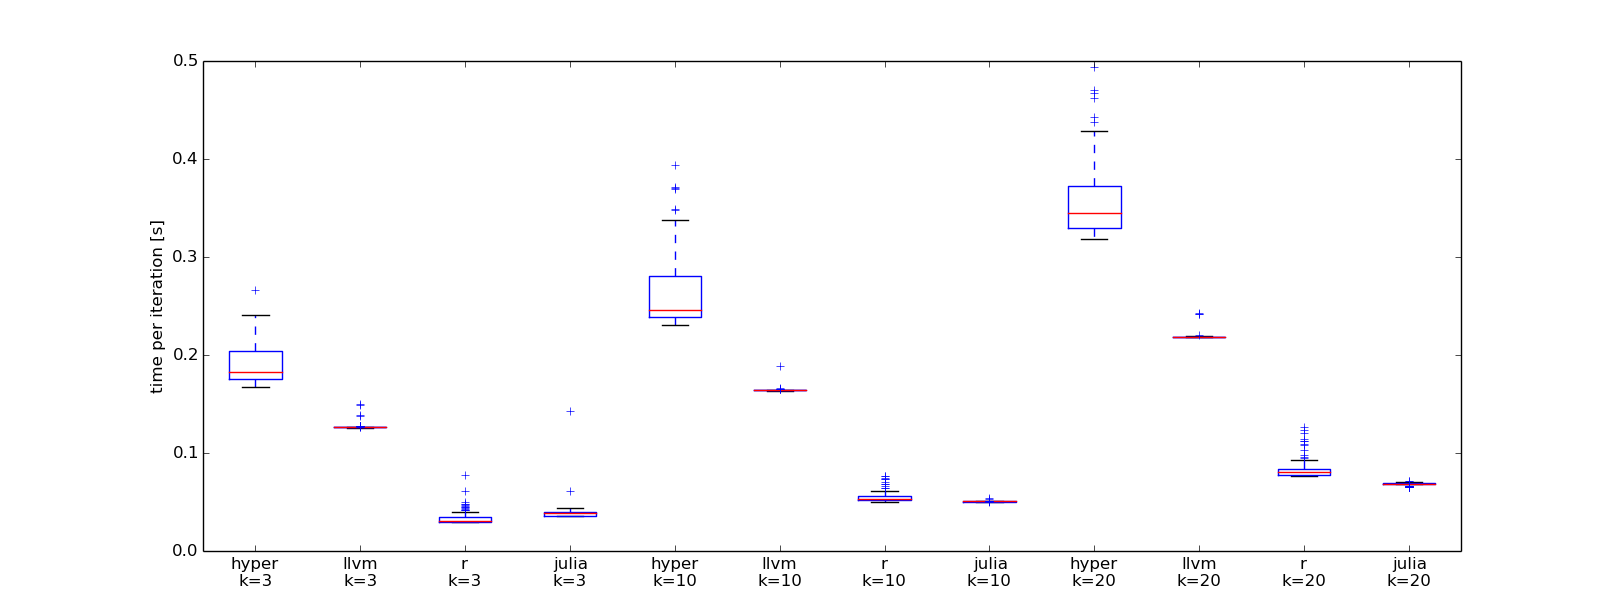
\includegraphics[scale=0.4, trim="0cm 1cm 0cm 0cm"]{figures/charts/50000_all}
  \caption[High Dimensional - Time per Iteration]{High Dimensional - Time per Iteration.}
  \label{fig:50000_all}
\end{figure}



Running the same experiment on the high dimensional data set we see a different result as depicted in~\autoref{tab:highdim_all}. As already shown, the HyPer C++ and the LLVM version are slower compared to the network data set even though the data set is smaller by size. R takes almost the same time for both data sets. Interestingly, Julia’s k-Means is now as fast as the R implementation, for $k = 10$ and 20 it is even faster.~\autoref{fig:50000_all} shows this results as a boxplot. 
\\
This result gives us interesting knowledge about the different implementations. Both HyPer operators perform poorly when dimensions increase. An increase in dimensions and a decrease in instances does not affect R significantly. On the other hand, Julia shows much better results as dimensions increases and seems to be optimized for high dimensions: It is 5.4, 4.4 and 4.2 faster for $k = 3, 10$ and 20 times on the high dimensional set compared to the network data. 

\begin{table}[htsb]
  \caption[Medium Size - Time per Iteration]{Medium Size - Time per Iteration.}
  \label{tab:medium_all}
  \centering
  \begin{tabular}{l l l l l l l l l l l l l}
    \toprule
      & \multicolumn{3}{c}{Julia} & \multicolumn{3}{c}{R} & \multicolumn{3}{c}{HyPer C++} & \multicolumn{3}{c}{HyPer LLVM}  \\
      k & 3 & 10 & 20 & 3 & 10 & 20 & 3 & 10 & 20 & 3 & 10 & 20 \\
    \midrule
      50  & 5.42 & 7.61 & 10.62 & 0.77 & 1.61 & 2.50 & 2.38 & 3.29 & 4.68 & 0.92 & 2.10 & 3.46 \\
      50  & 5.43 & 7.65 & 10.71 & 0.79 & 1.63 & 2.55 & 2.57 & 3.44 & 4.77 & 0.94 & 2.14 & 3.51 \\
      50  & 5.44 & 7.70 & 10.91 & 0.80 & 1.63 & 2.56 & 2.64 & 3.45 & 4.84 & 0.94 & 2.14 & 3.52 \\
    \bottomrule
  \end{tabular}
\end{table}

\begin{table}[htsb]
  \caption[Medium Size HD - Time per Iteration]{Medium Size HD - Time per Iteration.}
  \label{tab:medium_hd_all}
  \centering
  \begin{tabular}{l l l l l l l l l l l l l}
    \toprule
      & \multicolumn{3}{c}{Julia} & \multicolumn{3}{c}{R} & \multicolumn{3}{c}{HyPer C++} & \multicolumn{3}{c}{HyPer LLVM}  \\
      k & 3 & 10 & 20 & 3 & 10 & 20 & 3 & 10 & 20 & 3 & 10 & 20 \\
    \midrule
      50  & 11.46 & 15.69 & 21.67 & 9.43 & 15.48 & 23.77 & 16.39 & 34.12 & 59.40 & 10.42 & 22.11 & 38.80 \\
      50  & 11.51 & 15.81 & 21.69 & 9.50 & 15.50 & 23.79 & 16.77 & 36.11 & 59.53 & 10.44 & 22.12 & 38.84 \\
      50  & 11.65 & 15.83 & 21.70 & 9.64 & 15.58 & 23.79 & 17.29 & 42.15 & 59.57 & 10.45 & 22.13 & 38.84 \\
    \bottomrule
  \end{tabular}
\end{table}


\begin{figure}[htsb]
  \raggedleft
  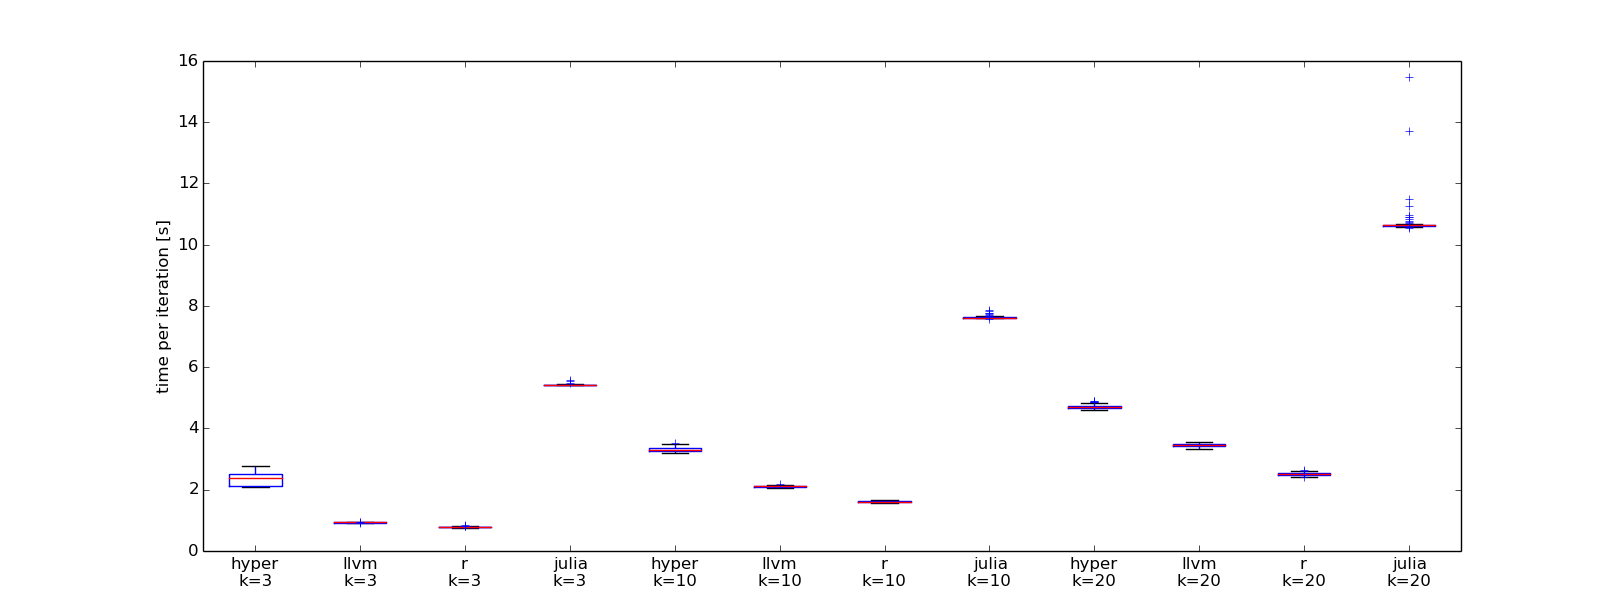
\includegraphics[scale=0.4, trim="0cm 1cm 0cm 0cm"]{figures/charts/15M_all}
  \caption[Medium Size - Time per Iteration]{Medium Size - Time per Iteration.}
  \label{fig:15M_all}
\end{figure}


\begin{figure}[htsb]
  \raggedleft
  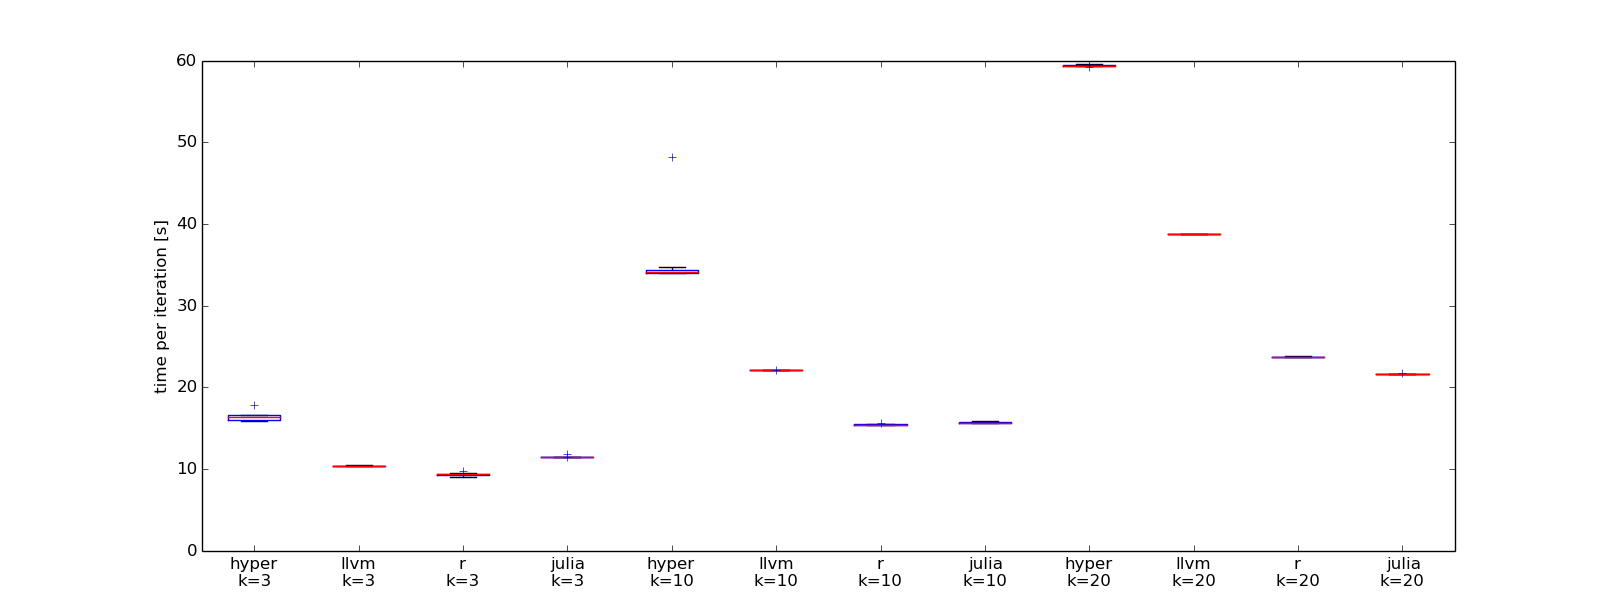
\includegraphics[scale=0.4, trim="0cm 1cm 0cm 0cm"]{figures/charts/15Mxhd_all}
  \caption[Medium Size HD - Time per Iteration]{Medium Size HD - Time per Iteration.}
  \label{fig:15Mxhd_all}
\end{figure}



We run the same experiment on the medium size and the medium size high dimensional data set.~\autoref{tab:medium_all} shows the results of the medium size data set. Again, the LLVM version is faster than the C++ version by a factor of 2.5, 1.6 and 1.4 for $k = 3, 10$ and $20$. Since the dataset has only four dimensions Julia performs poorly and is by a factor of 5.9, 3.6 and 3.1 slower compared to the LLVM version. As for the network data set R demonstrates the best performance and is faster than LLVM by a factor of 0.8 for $k = 3$ and 10 and 0.7 for $k = 20$.~\autoref{fig:15M_all} shows the results as a boxplot.
\\
For comparison~\autoref{tab:medium_hd_all} and ~\autoref{fig:15Mxhd_all} depict the result for the medium size high dimensional data set. As before, our own implementation does not perform ideally on high dimensions. For small $k = 3$, the LLVM version is slower than R by a factor of 0.9 but faster than Julia for a factor of 1.1. However, as $k$ grows, R and Julia show slightly better results. Both show a speed up by a factor of 0.7 for $k = 10$, and 0.6 for $k = 20$. 
\\
Obviously the high dimensional data set takes more time per iteration having a constant number of instances. Julia shows a slow down by a factor of 2 for all $k$'s, R by a factor of 12 for $k = 3$ and 10 for $k = 10$ and 20, the C++ version by a factor of 7, 10, 13 for $k = 3, 10$ and 20 and the LLVM version by a factor of 11 for all $k$'s. Julia perform again the best for high dimensional data. R and HyPer's LLVM operator behave very similar this time. An explanation is that the compilation time is not a limiting factor anymore for the LLVM implementation. For the high dimensional data set with 50000 instances the compilation time is higher than the execution time. This time the data set consists of 15 millions tuples therefore the poor compilation time does not affect the overall performance anymore.
\\
As final test we perform the same experiment on the large data set containing 150 million instances, as shown in~\autoref{tab:150M_all}. This time the HyPer LLVM implementation outnumbers all the other tools, the C++ version by a factor of 2.0, 1.5 and 1.4 for $k = 3, 10$ and 20, Julia by a factor of 3.6, 2.2, 2.0, respectively, and even R by a factor of 1.6, 1.2 and 1.1, respectively. This is also shown by a boxplot in~\autoref{fig:150M_all}. Julia's performance is quite compared to the other tools since the data set consist only of ten dimensions. For growing $k$, the R implementation comes very close to the HyPer LLVM version.
\\
In conclusion the experiments show that HyPer’s k-Means operator can compete with state-of-the-art tools for clustering. Particularly the LLVM implementation demonstrates a good performance and shows similar results to the R implementation of the k-Means algorithm. For high dimensional data sets the LLVM implementation does not perform ideally and is outnumbered by Julia's implementation optimized for high dimensions. If we take into account that the k-Means algorithm runs on top of an entire database with all its overhead, these results are affirmative for future development and the implementations of other operators on HyPer. 




\begin{table}[htsb]
  \caption[Large Size - Time per Iteration]{Large Size - Time per Iteration.}
  \label{tab:150M_all}
  \centering
  \begin{tabular}{l l l l l l l l l l l l l}
    \toprule
      & \multicolumn{3}{c}{Julia} & \multicolumn{3}{c}{R} & \multicolumn{3}{c}{HyPer C++} & \multicolumn{3}{c}{HyPer LLVM}  \\
      k & 3 & 10 & 20 & 3 & 10 & 20 & 3 & 10 & 20 & 3 & 10 & 20 \\
    \midrule
      50  & 65.62 & 90.37 & 132.39 & 29.47 & 48.21 & 72.40 & 37.29 & 62.01 & 92.60 & 18.38 & 40.49 & 67.25 \\
      50  & 65.72 & 92.01 & 135.87 & 30.80 & 54.73 & 77.27 & 37.50 & 62.41 & 92.86 & 18.44 & 40.72 & 67.57 \\
      50  & 65.78 & 92.27 & 137.21 & 33.08 & 55.02 & 77.97 & 37.52 & 62.72 & 92.95 & 18.46 & 40.72 & 67.63 \\
    \bottomrule
  \end{tabular}
\end{table}





\begin{figure}[htsb]
  \raggedleft
  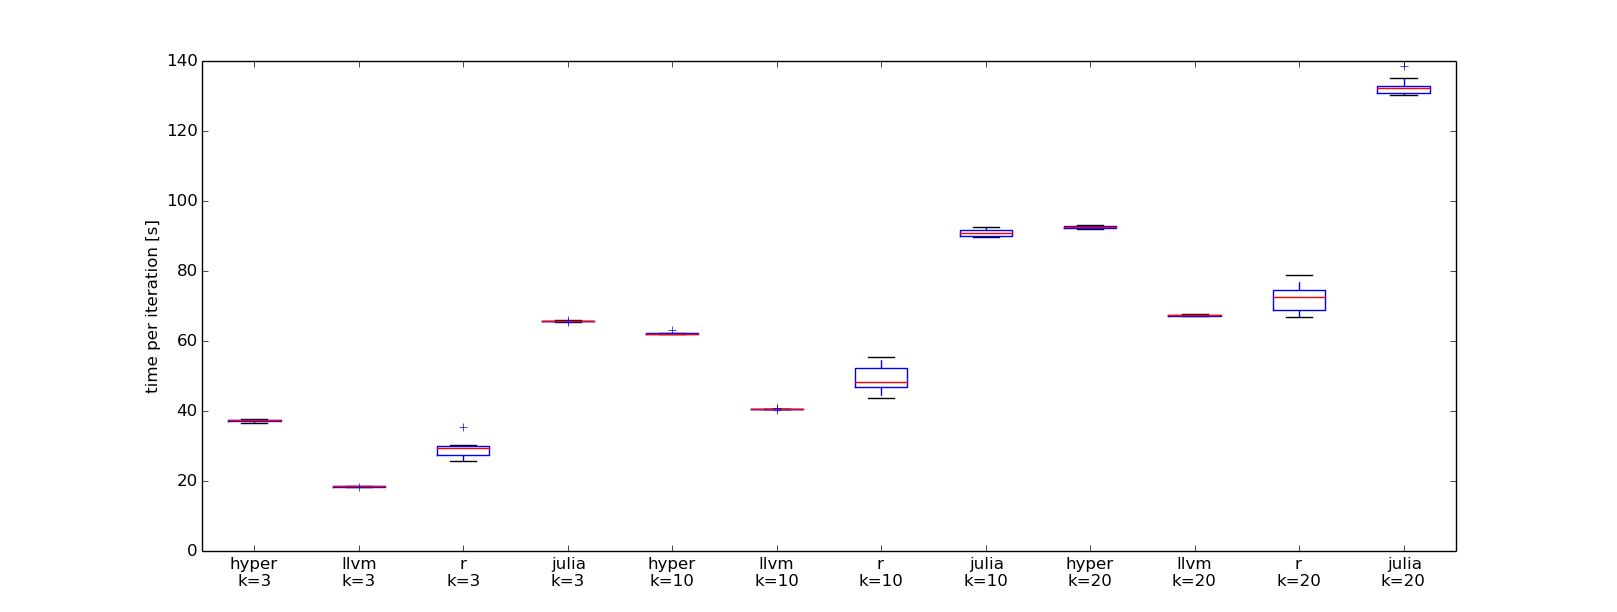
\includegraphics[scale=0.4, trim="0cm 1cm 0cm 0cm"]{figures/charts/150M_all}
  \caption[Large Size - Time per Iteration]{Large Size - Time per Iteration.}
  \label{fig:150M_all}
\end{figure}



\section{Parallel Implementation}


So far we only looked at the serial execution of the HyPer k-Means operator: In Section~\ref{section:serial}  we figured out that the LLVM implementation outperforms the C++ version on all used data sets. In Section~\ref{section:performance} we compared the performance against Julia and R and showed that HyPer is able to compete with state-of-the-art technologies for data mining.
\\
However as data sets grow serial execution takes more and more time, making real-time data mining almost impossible. Furthermore, we do not exploit the modern hardware of database systems and the advantages of multi-threaded execution. In this section we compare the parallel implementation of the HyPer k-Means operator with the LLVM version and the R implementation. Both tools demonstrate the best results on the medium size, the medium size high dimensional and the large data set. 

\begin{table}[htsb]
  \caption[Medium Size - Time per Iteration]{Medium Size - Time per Iteration.}
  \label{tab:medium_final}
  \centering
  \begin{tabular}{l l l l l l l l l l }
    \toprule
      & \multicolumn{3}{c}{R} & \multicolumn{3}{c}{HyPer LLVM} & \multicolumn{3}{c}{HyPer Parallel}  \\
      k & 3 & 10 & 20 & 3 & 10 & 20 & 3 & 10 & 20 \\
    \midrule
      50  & 0.77 & 1.61 & 2.50 & 0.92 & 2.10 & 3.46 & 1.35 & 1.52 & 1.75 \\
      90  & 0.79 & 1.63 & 2.55 & 0.94 & 2.14 & 3.51 & 1.38 & 1.53 & 1.84 \\
      95  & 0.80 & 1.63 & 2.56 & 0.94 & 2.14 & 3.52 & 1.40 & 1.53 & 1.85 \\
    \bottomrule
  \end{tabular}
\end{table}

~\autoref{tab:medium_final} shows the result as the time per iteration for $k = 3, 10$ and 20. As before, the median, the 90th and 95th percentile are presented. For $k = 3$, we see that both the R and the LLVM version are faster than the parallel version. However, as k grows, the parallel version outperforms R and the LLVM version. This circumstance is also shown in the bar chart in~\autoref{fig:final_15M}.
\\
The reason is that for the parallel execution the running time is almost independent of $k$, threfore the parallel version outperforms R and LLVM: For R, the time per iterations grows by a factor of 2.1 from $k = 3$ to $k = 10$, and by a factor of 1.6 from $k = 10$ to $k = 20$, and for LLVM by a factor of 2.3 and 1.6, respectively. In contrast, the parallel implementation grows only by factor of 1.1 and 1.2, respectively. Therefore, R and the LLVM version grow by seconds as $k$ grows, while the parallel version grows insignificantly by around 200 milliseconds. 

\begin{figure}[htsb]
  \centering
  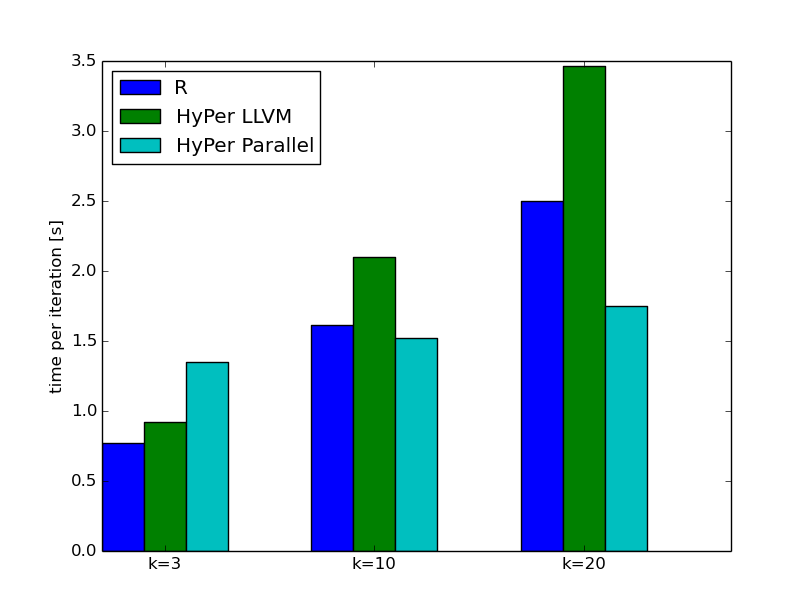
\includegraphics[scale=0.4, trim="0cm 1.5cm 0cm 0cm"]{figures/charts/final_15M}
  \caption[Medium Size - Time per Iteration]{Medium Size - Time per Iteration.}
  \label{fig:final_15M}
\end{figure}

~\autoref{tab:medium_hd_final} shows the same experiment on the medium high dimensional data set. For this data set the parallel version outperforms the other two implementations for all $k$'s, even for $k = 3$.~\autoref{fig:final_15_hd} depicts that the parallel version in again almost independent of $k$, in contrast to R and LLVM: R grows by a factor of 1.6 from $k = 3$ to $k = 10$, and 1.5 from $k = 10$ to $k = 20$, and for LLVM 2.1 and 1.8, respectively. The parallel version starts at low 5.84 seconds and grows by a factor 1.4 from $k = 10$ and $k = 20$. 
\\
So this time, the parallel version not as independent by the cluster number $k$ as for the low dimensional data set of same size. Instead, the performance gain results in the ability to handle high dimensional data better: From four dimensions to 50 dimension, the parallel execution time is only affected by a factor of 4.3, 5.3 and 6.5 for $k = 3, 10$ and 20. R and LLVM are affected by a much higher factor: 12.3, 9.6 and 9.5 for R, 11.3, 10.5 and 11.2 for the LLVM implementation. Only the for high dimensions optimized Julia shows with a factor of 2.1, 2.1 and 2.0 better results.

\begin{table}[htsb]
  \caption[Medium Size HD - Time per Iteration]{Medium Size HD - Time per Iteration.}
  \label{tab:medium_hd_final}
  \centering
  \begin{tabular}{l l l l l l l l l l }
    \toprule
      & \multicolumn{3}{c}{R} & \multicolumn{3}{c}{HyPer LLVM} & \multicolumn{3}{c}{HyPer Parallel}  \\
      k & 3 & 10 & 20 & 3 & 10 & 20 & 3 & 10 & 20 \\
    \midrule
      50  & 9.43 & 15.48 & 23.77 & 10.42 & 22.11 & 38.80 & 5.84 & 8.04 & 11.30 \\
      90  & 9.50 & 15.50 & 23.79 & 10.44 & 22.12 & 38.84 & 5.88 & 8.26 & 11.35 \\
      95  & 9.64 & 15.58 & 23.79 & 10.45 & 22.13 & 38.84 & 5.88 & 8.29 & 11.37 \\
    \bottomrule
  \end{tabular}
\end{table}



\begin{figure}[htsb]
  \centering
  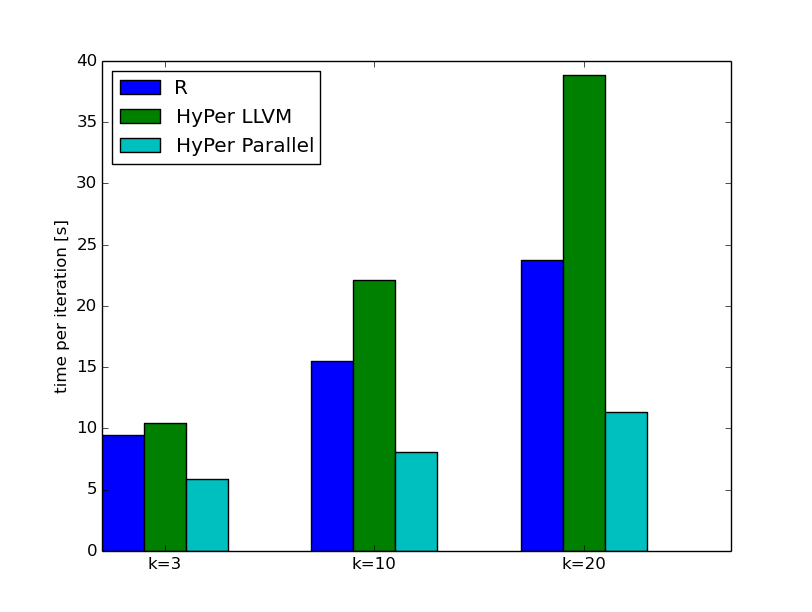
\includegraphics[scale=0.4, trim="0cm 1.5cm 0cm 0cm"]{figures/charts/15Mxhd_final}
  \caption[Medium Size HD - Time per Iteration]{Medium Size HD - Time per Iteration.}
  \label{fig:final_15_hd}
\end{figure}

Finally,~\autoref{tab:large_final} shows the results of the same experiment on the large data set. Again, the parallel is the fastest. For $k = 3$, the parallel version is faster than R by a factor of 1.8 and for LLVM by a factor of 1.1. For $k = 10$ the factor is even larger, 2.4 for R and 2.0 for LLVM, and 3.0 and 2.8 for $k = 20$, respectively. Since $k$ affects the performance of the parallel version only slightly, the factor is increasing as $k$ increases.
\\
To conclude, except for the medium size data set and $k = 3$ the parallel version is much better than the LLVM and R algorithm. However, since we are using 16 cores even a higher speed up would be possible. As explanation, we have to take into account the overhead of the parallel process. Furthermore, we are using the slower C++ version of the HyPer k-Means operator as foundation for our parallel implementation. Even though parts of the algorithm are parallelized, we still have all the downsides of many function calls between the runtime and the compile time system and of the high-level C++ constructs. And finally, we parallize only the computation of the distances, not the cluster update.


\begin{table}[htsb]
  \caption[Large Size - Time per Iteration]{Large Size - Time per Iteration.}
  \label{tab:large_final}
  \centering
  \begin{tabular}{l l l l l l l l l l }
    \toprule
      & \multicolumn{3}{c}{R} & \multicolumn{3}{c}{HyPer LLVM} & \multicolumn{3}{c}{HyPer Parallel}  \\
      k & 3 & 10 & 20 & 3 & 10 & 20 & 3 & 10 & 20 \\
    \midrule
      50  & 29.47 & 48.21 & 72.40 & 18.38 & 40.49 & 67.25 & 16.71 & 19.79 & 24.03 \\
      90  & 30.80 & 54.73 & 77.27 & 18.44 & 40.72 & 67.57 & 16.94 & 20.13 & 24.33 \\
      95  & 33.08 & 55.02 & 77.97 & 18.46 & 40.72 & 67.63 & 17.01 & 20.17 & 24.36 \\
    \bottomrule
  \end{tabular}
\end{table}




\begin{figure}[htsb]
  \centering
  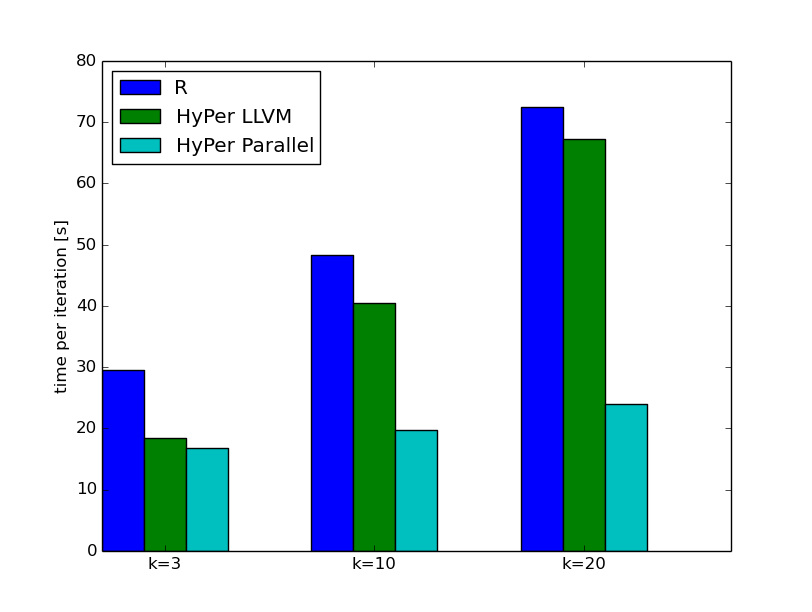
\includegraphics[scale=0.4, trim="0cm 1.5cm 0cm 0cm"]{figures/charts/final_150M}
  \caption[Large Size - Time per Iteration]{Large Size - Time per Iteration.}
  \label{fig:final_150M}
\end{figure}


